\documentclass[dvipsnames,beamer,10pt]{standalone}

\usepackage{tikz}
\usetikzlibrary{positioning,decorations.pathreplacing,fit}
\usetikzlibrary{decorations.markings,arrows.meta,shapes.arrows,arrows}
\usetikzlibrary{calc}

\definecolor{mygreen}{RGB}{0,128,80}
\colorlet{darkgreen}{mygreen!90!black}


%\makeatletter
%\DeclareMathSizes{\f@size}{5}{5}{5}
%\makeatother

\DeclareMathSizes{10.0}{10}{5}{5}

\providecommand{\dlog}[2]{\textcolor{#1}{#2}}
\providecommand{\ua}[1]{\dlog{red}{#1}}
\providecommand{\ub}[1]{\dlog{blue}{#1}}
\providecommand{\uc}[1]{\dlog{Plum}{#1}}
\providecommand{\ud}[1]{\dlog{OliveGreen}{#1}}
\providecommand{\oracle}[2]{\pi_{\hspace*{-1pt}#1}^{#2}}

\begin{document}

%\small





\begin{standaloneframe}

\resizebox{1\textwidth}{!}{



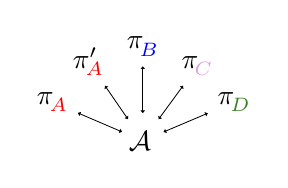
\begin{tikzpicture}[
	send/.style= {
		>={Latex[length=1pt,width=1.8pt]},<->,shorten <= 1pt,line width=0.3pt
	},
	]

	

	\node[] (A) {\hspace*{-2pt}$\mathcal{A}$};
	
	\node[above left = 0pt and 17pt of A] (s1) {$\oracle{\ua{A}}{}$};
	\node[above left = 13pt and 4pt of A] (s2) {$\oracle{\ua{A}}{\prime}$};
	\node[above = 20pt of A] (s3) {$\oracle{\ub{B}}{}$};
	\node[above right = 13pt and 4pt of A] (s4) {$\oracle{\uc{C}}{}$};
%	\node[above right = 13pt and 4pt of A] (s4) {$\alt<+(1)>{\ua{\oracle{\uc{C}}{}}}{\oracle{\uc{C}}{}}$};
	\node[above right = 0pt and 17pt of A] (s5) {$\oracle{\ud{D}}{}$};
	
	\draw[send] (A) -- (s1);
	\draw[send] (A) -- (s2);
	\draw[send,shorten <= 3pt] (A) -- (s3);
	\draw[send] (A) -- (s4);
	\draw[send] (A) -- (s5);
	
 

\end{tikzpicture}


}

\end{standaloneframe}


\end{document}